\documentclass[11pt]{article}
\usepackage[margin=1in]{geometry}
\usepackage{amsmath,amssymb}
\usepackage{booktabs}
\usepackage{multirow}
\usepackage{enumitem}
\usepackage[expansion=false]{microtype}
\usepackage[hidelinks]{hyperref}
\usepackage{xcolor}
\usepackage{tikz}
\usetikzlibrary{arrows.meta,positioning,fit,backgrounds}

\newcommand{\aims}{\textsc{Aims}}
\newcommand{\best}[1]{\textbf{#1}}

\title{\textbf{Design as the Objective:\\ Why an LLM Must Be Given the Structure It Should Produce,\\ and a Blind Evaluation of a Method That Does}}

\author{Eliezer Avihail\\ \texttt{github.com/eliezeravihail/aims}}
\date{September 2026}

\begin{document}
\maketitle

\begin{abstract}
A language model optimizes the objective it is given, not the instructions it is handed. Coding agents are scored --- in training, in benchmarks, and in the closing condition of every agent loop --- on functional correctness. Architectural quality is therefore never an objective; it is at best a stylistic prior, and it loses to the immediate task. We argue from the mechanics of autoregressive generation and preference optimization that this is a structural property rather than a capability gap, and that three consequences follow: a quality goal must be stated as a checkable predicate rather than an adjective; it must be checked at the moment a structural decision is made, because generation is path-dependent and a model conditioned on an interface it has already written will rationalize rather than revise it; and the rationale must be externalized into durable artifacts, because the model is stateless across sessions.

We present \aims{}, a method for terminal coding agents built on those three consequences: a Guide sets one design objective per round and delegates to Workers; two principle documents define what ``correct'' means for building from nothing and for changing existing code; one measurement instrument scores every item as a cited binary sub-check with severity-derived ceilings and weights; and design conclusions are filed as records co-located with the code, anchored by content hash and re-surfaced by advisory hooks.

We evaluate the shipped method under a frozen adversarial protocol --- staged requirement cards that never hint at later stages, a strict passive oracle, method-anonymized artifacts, blind judges with sealed mappings and a reproduction required for every load-bearing claim. Against a spec-driven baseline on three fresh products, \aims{} wins first-round design quality on all three on a single recurring axis (value objects and one-owner-per-rule), while change absorption is tie / win / tie on the rubric-free count and both arms pass every correctness trap. Across six adaptation experiments --- including one on a real open-source module --- a no-method control is correct every time; the method's measurable edge is a design trajectory that improves across successive changes while the control flattens and densifies. Costs are 2.5--3$\times$ the baseline (1.9--2.3$\times$ in a follow-up). A follow-up campaign finds that an identical passing test suite never separated designs the rubric scored 43 against 16; that what catches a design which passes every test yet is badly built is the method's \emph{review} of the output, not its principles placed in the prompt; and that the one measured outcome of the co-located record is a declared non-goal, which the code cannot carry (3 of 3 agents with the record caught a change that contradicted it, 0 of 3 without). A test at scale --- three successive cross-cutting changes to a 7,000-line open-source codebase, chosen only after a gate showed that unaided agents sometimes get its design wrong --- finds the method's designs scored above unaided ones at every stage by blind judges, with the method's records withheld; the final-stage verdict holds under two of three judges and rests on a correction to the judges' specification that we report in full. The same test finds the record's value in the same place as before: every session given the record surfaced a contradicted legal non-goal (3 of 3 sessions), against 2 of 3 and 1 of 3 without it --- one short of the threshold we registered. We report two results that are not wins: a perfect first-round score on all three products, which we read as a ceiling effect that removes the instrument's ability to detect the next regression, and independent observations by all three judges that the method's designs speak the rubric's own vocabulary. Finally we show, on the only pair of runnable arms available, that every deterministic static metric is blind to --- and two are anti-correlated with --- the design difference a blind judge penalized, and argue that architectural evaluation is therefore necessarily an instrument of procedure rather than of measurement.
\end{abstract}

\section{Introduction}

Give a competent coding agent a repository and a requirement and it will usually produce something that works. Give it twenty requirements in sequence, each in a fresh session, and the artifact decays in a characteristic way: each change is locally reasonable, the tests keep passing, and the structure degrades --- one concept modelled two ways, an interface calibrated for one kind of thing quietly absorbing a foreign one, a rule that had one owner acquiring a second. The cost lands on the \emph{next} change and is invisible to any predicate evaluated now. This is the problem Parnas identified at the origin of modular design~\cite{parnas1972criteria}, and it has not become easier because the author is a model.

The usual reading is that this is a capability gap to be closed by better models. We argue in Section~\ref{sec:mechanism} that it is not: it follows from what an LLM is optimizing at inference time and from what its training signal rewards. The argument yields three design requirements, and \aims{} (``AI Manager System'') is an instantiation of them. Sections~\ref{sec:related}--\ref{sec:method} place the method against prior and competing work and describe it; Sections~\ref{sec:protocol}--\ref{sec:results} give the protocol and the current results; Section~\ref{sec:measurement} reports why we cannot offer the deterministic benchmark the reader will want.

\section{Why a Language Model Produces the Structure It Produces}
\label{sec:mechanism}

\subsection{What is actually being optimized}

A transformer language model~\cite{vaswani2017attention} defines a conditional distribution over continuations, $p_\theta(x_t \mid x_{<t})$, and generation samples from it token by token. At inference there is no search over programs and no objective function over the finished artifact: the only quantity being maximized, locally, is the likelihood of the next token given everything already in the context. Whatever ``goal'' the model pursues is a property of that conditioning --- it is the goal the \emph{prompt makes probable}, realized through in-context learning~\cite{brown2020language}.

Instruction tuning and preference optimization~\cite{ouyang2022training} shape which continuations are likely by rewarding outputs that human raters prefer. This is where the relevant distortion enters. Raters --- and the preference models trained on them --- reward responses that \emph{appear} to satisfy the request. Sharma et al.~\cite{sharma2023sycophancy} show empirically that this incentive is strong enough to make preference-trained assistants favour agreement with the user over truth across several production models, and that preference models sometimes prefer a convincingly written wrong answer to a correct one. The general form is older than LLMs: an optimizer satisfies the literal specification it is scored against, not the outcome the specifier intended --- specification gaming~\cite{krakovna2020specification}, reward hacking~\cite{amodei2016concrete}, Goodhart's law in its formal variants~\cite{manheim2019categorizing}.

Now consider what the standard coding-agent loop actually scores. The benchmarks that legitimized the capability --- HumanEval~\cite{chen2021codex}, MBPP~\cite{austin2021program}, SWE-bench~\cite{jimenez2024swebench} --- close on a functional predicate. Agent scaffolds inherit it: ReAct~\cite{yao2023react} interleaves reasoning and action until the task is done; Self-Refine~\cite{madaan2023selfrefine} and Reflexion~\cite{shinn2023reflexion} add a critic that shares the actor's objective; SWE-agent~\cite{yang2024sweagent} operationalizes this at repository scale. In every case the loop's terminal condition is \emph{it works}.

\paragraph{Consequence 1: an adjective is not an objective.} ``Write clean, well-architected code'' adds tokens that raise the probability of text \emph{about} good structure, and of the shallow surface features of it, without adding any predicate the generation can fail. The model has no way to distinguish a satisfied constraint from an unsatisfied one, so the phrase behaves as style conditioning rather than as a goal. A structural goal becomes real only when it is stated as something checkable --- an enumerable list of items, each of which a reader can answer yes or no about, with the check applied to the output. This is the single assumption \aims{} rests on: \emph{a model optimizes the goal it is given, not the instructions it is handed}; so if correct structure is wanted, structure must be the goal, and there must exist a document that says what ``correct'' means.

\subsection{Why the check must fire at the decision, not after it}

Autoregressive generation is path-dependent in a way that matters here. Once the model has emitted an interface, every subsequent token is conditioned on it; the interface is now part of the evidence the model is explaining. Asking afterwards ``is this interface right?'' poses a question whose most probable continuation is a defence, because the context contains a designed artifact plus the model's own reasons for it. Self-critique scaffolds~\cite{madaan2023selfrefine,shinn2023reflexion} work well where the error is locally visible (a failing test, a type error) and poorly where the error is a commitment the whole context is built on.

There is a second, simpler asymmetry: a design defect costs a paragraph to fix before the code exists and a refactor afterwards. Both point the same way --- the structural check belongs \emph{inside} the design step, before the artifact conditions the rest of the generation. Section~\ref{sec:results} contains a direct instance: a concept-fit check that was already written in the method's own principles fired only at review time and did not prevent the fault; moved to the design step, it eliminated it.

\paragraph{Consequence 2: check at design time, with the design as the artifact under test.}

\subsection{Why rationale has to leave the context window}

A model has no memory between sessions. Within a session its state is the context window, and even there attention to material in the middle of a long context degrades measurably~\cite{liu2024lost}. The practical effect is that the \emph{reasons} for a boundary --- what was considered and rejected, what invariant the seam protects --- exist only as tokens that are discarded when the session ends. A later session sees the code but not the why, cannot distinguish a deliberate boundary from an accident, and will dissolve the former with the same confidence it would remove the latter.

This is the problem Architecture Decision Records~\cite{nygard2011adr} solve for human teams and literate programming~\cite{knuth1984literate} argues for generally, but the agent setting adds a hazard neither anticipated: the reader is a system with a strong prior toward treating supplied text as true. A stale record is therefore worse than no record --- it will be followed. Any durable-knowledge scheme for agents needs a staleness signal as a first-class part of the design, not a documentation practice.

\paragraph{Consequence 3: externalize the rationale next to the artifact, and detect when it has gone stale.}

\subsection{Why the default attractor is under-structuring}

The prior a code model brings is the distribution of its training corpus, which is dominated by working code of ordinary quality: flat procedures, inline literals, primitives standing in for concepts, data bags with the logic elsewhere, rules enforced in no particular place. Under a correctness-terminated loop, nothing pulls away from that median. Over-engineering is possible and does occur, but it is a \emph{local} cost --- a layer nobody uses --- whereas under-structuring spreads, because every later change must route around the missing seam. \aims{} encodes this asymmetry explicitly: when unsure, the graver risk is too little structure, and the over-build/under-provision severity split in Section~\ref{sec:method} is the mechanical form of it.

\begin{figure}[t]
\centering
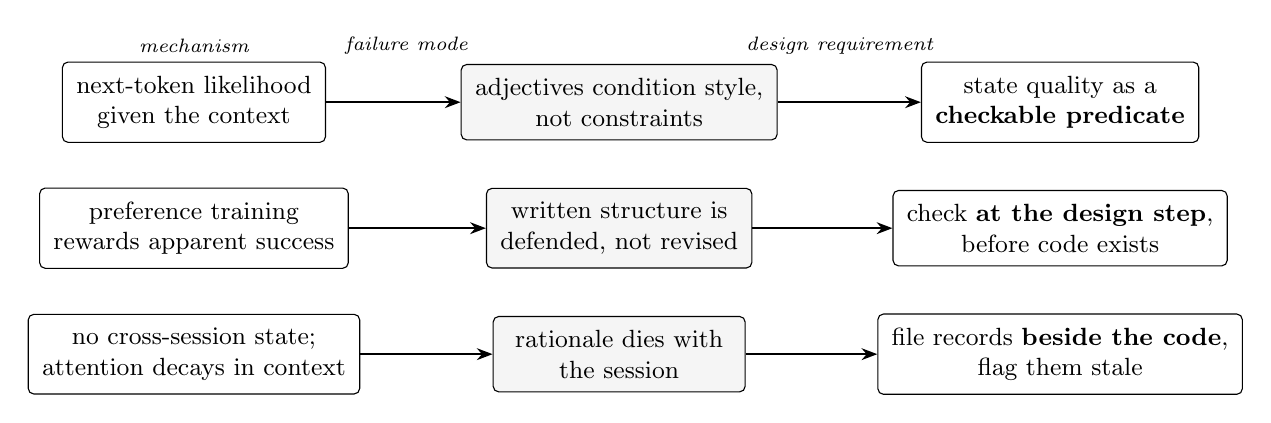
\begin{tikzpicture}[
  font=\small,
  b/.style={draw, rounded corners=2pt, align=center, inner sep=5pt, minimum height=9mm},
  lbl/.style={font=\scriptsize\itshape},
  arr/.style={-{Stealth[length=2mm]}, thick}
]
\node[b, minimum width=30mm] (mech1) at (0,0) {next-token likelihood\\ given the context};
\node[b, minimum width=30mm] (mech2) at (0,-1.6) {preference training\\ rewards apparent success};
\node[b, minimum width=30mm] (mech3) at (0,-3.2) {no cross-session state;\\ attention decays in context};
\node[b, minimum width=32mm, fill=black!4] (f1) at (5.4,0) {adjectives condition style,\\ not constraints};
\node[b, minimum width=32mm, fill=black!4] (f2) at (5.4,-1.6) {written structure is\\ defended, not revised};
\node[b, minimum width=32mm, fill=black!4] (f3) at (5.4,-3.2) {rationale dies with\\ the session};
\node[b, minimum width=34mm] (r1) at (11.0,0) {state quality as a\\ \textbf{checkable predicate}};
\node[b, minimum width=34mm] (r2) at (11.0,-1.6) {check \textbf{at the design step},\\ before code exists};
\node[b, minimum width=34mm] (r3) at (11.0,-3.2) {file records \textbf{beside the code},\\ flag them stale};
\draw[arr] (mech1) -- (f1); \draw[arr] (mech2) -- (f2); \draw[arr] (mech3) -- (f3);
\draw[arr] (f1) -- (r1); \draw[arr] (f2) -- (r2); \draw[arr] (f3) -- (r3);
\node[lbl] at (2.7,0.72) {failure mode};
\node[lbl] at (8.2,0.72) {design requirement};
\node[lbl, align=center] at (0,0.72) {mechanism};
\end{tikzpicture}
\caption{The argument of Section~\ref{sec:mechanism}. Each row is a property of how the model generates, the failure it produces under a correctness-terminated loop, and the requirement it imposes on any method that wants structure as an outcome.}
\label{fig:argument}
\end{figure}

\section{Prior and Competing Methods}
\label{sec:related}

\paragraph{Single-agent scaffolds.} ReAct~\cite{yao2023react} is the substrate for most coding agents. Self-Refine~\cite{madaan2023selfrefine} and Reflexion~\cite{shinn2023reflexion} add reflection, and SWE-agent~\cite{yang2024sweagent} adds an agent-computer interface for repository-scale work. All terminate on task success; none carries a definition of structural quality, and by the argument of Section~\ref{sec:mechanism} their critic step is applied at the point where revision is least likely.

\paragraph{Multi-role frameworks.} AutoGen~\cite{wu2023autogen} and ChatDev~\cite{qian2024chatdev} distribute work across roles that imitate a software organization. MetaGPT~\cite{hong2024metagpt} sharpens this by having roles exchange \emph{standardized documents} rather than free-form chat, and is the closest antecedent to the Guide/Worker split used here. The difference is purpose: in those systems the split divides labour to complete the task, and the architect role exists to produce a design faster. In \aims{} the split exists to create a commitment barrier and to instantiate Consequence~2 --- the planning role's terminal act is to file a design record and stop, and the building role's authority derives from that record rather than from a conversation.

\paragraph{Spec-driven development.} OpenSpec, GitHub's Spec Kit and Kiro's spec mode route agent work through requirements $\rightarrow$ design $\rightarrow$ tasks with approval gates. This family is the serious competitor and is our baseline. It satisfies Consequence~2 partially --- there is a design step --- but the unit is the \emph{change}: a spec describes a delta, is consumed by implementation, and is archived. It carries no definition of structural quality against which the design step is scored, and it does not satisfy Consequence~3, since nothing durable remains attached to the artifact. \aims{}'s unit is the artifact, and its design step is scored against an explicit document.

\paragraph{Design rationale and knowledge.} ADRs~\cite{nygard2011adr} and literate programming~\cite{knuth1984literate} are the ancestors of the record layer; both assume a human reader who notices when documentation and code disagree, which is why anchoring and a staleness signal are additions rather than refinements.

\paragraph{Refactoring and legacy practice.} The brownfield half of the method is drawn from established practice: separate the behaviour-preserving step from the behaviour-changing one (``make the change easy, then make the easy change''~\cite{beck2012tweet}); characterize existing behaviour before touching it, and work through seams~\cite{feathers2004working}; name the smell being removed from a catalogue~\cite{fowler2018refactoring}. Our contribution here is not the practice but making it a scored checklist with correctness classes, and measuring it as a \emph{delta on the target} rather than against an abstract ideal.

\paragraph{Structural metrics.} The classical vocabulary --- cyclomatic complexity~\cite{mccabe1976complexity}, the CK suite~\cite{chidamber1994metrics}, Martin's package metrics~\cite{martin2003agile}, Halstead volume~\cite{halstead1977elements} and the derived Maintainability Index~\cite{coleman1994using} --- is what one would reach for as an objective benchmark. Section~\ref{sec:measurement} reports why it does not serve here. The alternative in current practice, LLM-as-judge~\cite{zheng2023judging}, brings its own failure modes, two of which we observed and quantify in Section~\ref{sec:threats}.

\section{The \aims{} Method}
\label{sec:method}

\aims{} installs as a plugin beside a terminal coding agent's native mechanisms, adding skills, commands and two advisory hooks, and replacing nothing.

\subsection{Roles}
The \textbf{Guide} selects \emph{one} design objective for the round and delegates execution to \textbf{Workers}. For an opening round the method may fan out a panel: three axis-focused Workers --- clean code, correct encapsulation, correct genericity --- design independently against the shared objective, no Worker seeing another's output, and a \textbf{merge agent} composes the best from each axis at full strength. The merge is explicitly not a winner-pick, a union or an average: strengths stay attributable to their Worker, merge-authored content is limited to integration glue, and irreconcilable conflicts are decided with a stated reason. Ordinary rounds use a single planning pass, and every planning round ends with one mandatory review-and-revise cycle against the instrument below.

\subsection{Two documents define ``correct''}
\label{sec:principles}
One document is the single source of correctness; the build instructions, the review, the fix-list and the grading all \emph{read} it and none defines correctness on its own.

\emph{Design principles} (fifteen chapters, \S0--\S14) covers building from nothing. Each chapter is a list of individually checkable items, and each item carries a \textbf{correctness class} that the scoring reads rather than redefines: \emph{preconditions}, whose violation makes the code wrong rather than untidy (functional correctness and contracts; one-owner-per-rule; module-seam leaks; concurrency safety under real concurrency; security where a trust boundary exists); \emph{conditional} items scored only against a stated requirement; \emph{code-leaning} items that are N/A on a pure design document; and \emph{quality} items, scored by pervasiveness. A foundational chapter on encapsulation and module seams is declared to dominate the rest and carries the heaviest weight.

Three elements of this document are design decisions rather than prose, and each traces to a measured failure:
\begin{itemize}[leftmargin=*,itemsep=2pt]
\item \textbf{The full-input-space trace.} Correctness is not ``every stated acceptance case'' but every case \emph{plus}, for each change-axis crossed with each rule, the interaction it implies --- stated as a procedure, because the failure it prevents is exactly a required output that no listed case exercises.
\item \textbf{Concept fit.} Model a thing as the kind it \emph{is}, not as a degenerate or synthetic instance of a neighbouring type. The cram is value-correct and concept-wrong, so it passes every test and breaks only under a later change; its tell is always an inert stand-in. The check is generalized over the family --- a decomposition forced into a movement, a distinct concept forced into a neighbouring entity, a first-class effect modelled as the absence of another, a filter modelled as a score --- and it runs on the design, before code (Consequence~2).
\item \textbf{A registered tie-break} between ``add a seam when in doubt'' and ``cut what pays for nothing''. When they collide on the same element, resolve by the change-axes, with deliberately asymmetric severity: a seam no foreseeable change-axis item would use is over-build, capped at the lowest tier; a seam a foreseeable item would force open is under-provision at a high tier. The falsifier is explicit --- name the change-axis item the seam serves. Registering it removes the structure-versus-minimalism call from a judge's taste, which is precisely where two reasonable judges diverge.
\end{itemize}

\emph{Add-feature principles} (12 chapters) is the brownfield companion, on the argument that adapting existing code is a different task with different dominant risks: greenfield's danger is too little structure, while a change's dangers are silent behaviour drift, editing code nobody characterized, scattering a rule while patching it, and bolting a requirement on instead of reshaping to absorb it. Its preconditions are characterize-before-touch, bit-for-bit preservation of what is out of scope, survival of one-owner through the change, and re-tracing the interaction where the change crosses an existing rule. Two of its rules govern how it is evaluated: its \textbf{measure is a before-and-after review on the target's own terms} --- no regression on \emph{this} module, with the trajectory across successive changes mattering more than any single step, because rot is cumulative and every step ``works''; and its \textbf{overriding constraint is consistency over dogma} --- adapt to the existing code's grain even where that contradicts a principle in either document, because importing a foreign style into a plain module is itself a regression. The goal is no new mess, not conformance to the list.

\subsection{One measurement instrument}
\label{sec:instrument}

The in-loop review, the standalone review command and any comparison of designs fill the same form (Figure~\ref{fig:instrument}). Chapters are rows; a chapter's items are its binary, cited sub-checks; $\textrm{chapter score} = \mathrm{round}(10 \times \textrm{items passed} / \textrm{items applicable})$.

Applicability is fixed at \emph{step 0}, before any scoring, by pinning from the specification --- never from the design --- the rules and invariants (R), the change-axes plus one plausible unstated variant (X), and the acceptance cases (C). Every failed sub-check must cite an R/X/C item or a named seam; an uncited finding is not counted; one defect is scored under one item only, which is what prevents a long checklist from double-counting a single fault.

Severity follows the failed item's correctness class and sets both a ceiling and a weight (Table~\ref{tab:severity}). The reported grade is the weighted list over chapters; severity is published beside it as a \emph{gate} --- any precondition (S4) failure marks the design \textsc{blocked} until it is fixed --- together with the worst chapter and the counts of structural and precondition failures, never a bare number.\footnote{The evaluation in Section~\ref{sec:results} was run under an earlier form of the instrument that additionally applied a global graded cap (any S2 $\leq 8.5$, S3 $\leq 7.5$, S4 $\leq 5.0$) by \texttt{min}. That cap was removed because it double-counted a single defect --- once through the chapter ceiling, again through the chapter weight, and a third time through the cap --- and was replaced by the reported gate above, applied retroactively to every prior experiment with both readings kept side by side. The Study~1 grades are unaffected where a chapter's worst item is cosmetic and are lower bounds otherwise; no ranking reported here changes.} Because applicability is fixed by step 0 from the specification, \textbf{all arms of one product share the same applicable set and are directly comparable, while grades across different products are not} and are never read as a single verdict on the method.

Two projections of the same filled form exist: a \emph{fix-list} with no aggregate shown for the build side --- deliberately, so a Worker fixes findings rather than a number --- and the full scored profile for comparing designs.

\begin{table}[h]
\centering\small
\caption{Severity mechanics. The tier of a chapter's worst failed item sets its ceiling and its weight in the aggregate.}
\label{tab:severity}
\begin{tabular}{lcc}
\toprule
Worst failed item in the chapter & Ceiling & Weight \\
\midrule
none & 10 & $\times$1 \\
cosmetic (S1) & 8 & $\times$1 \\
moderate (S2) & 7 & $\times$2 \\
structural (S3) & 5 & $\times$4 \\
precondition / correctness (S4) & 2 & $\times$8 \\
\midrule
\multicolumn{3}{l}{\emph{Reported gate (beside the grade, not a cap on it):} any S4 $\Rightarrow$ \textsc{blocked} until the precondition is fixed} \\
\bottomrule
\end{tabular}
\end{table}

\begin{figure}[t]
\centering
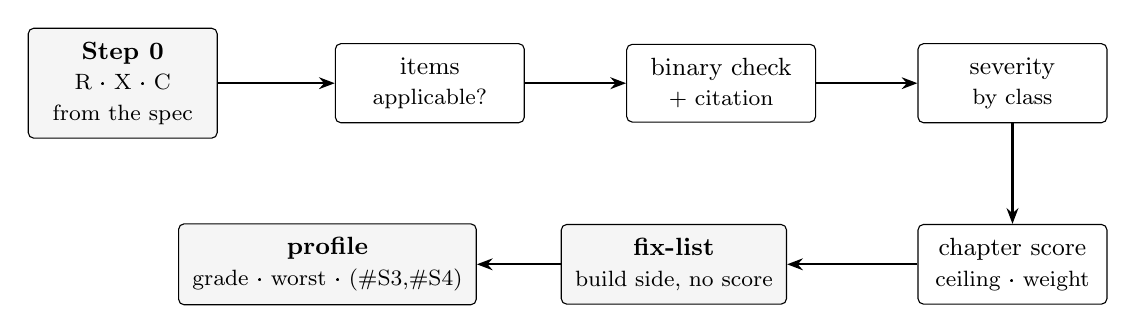
\begin{tikzpicture}[
  font=\small,
  b/.style={draw, rounded corners=2pt, align=center, inner sep=5pt, minimum height=9mm, minimum width=24mm},
  arr/.style={-{Stealth[length=2mm]}, thick}
]
\node[b, fill=black!4] (spec) at (0,0) {\textbf{Step 0}\\ \footnotesize R · X · C\\ \footnotesize from the spec};
\node[b] (items) at (3.9,0) {items\\ \footnotesize applicable?};
\node[b] (check) at (7.6,0) {binary check\\ \footnotesize + citation};
\node[b] (sev) at (11.3,0) {severity\\ \footnotesize by class};
\node[b] (row) at (11.3,-2.3) {chapter score\\ \footnotesize ceiling · weight};
\node[b, fill=black!4] (fix) at (7.0,-2.3) {\textbf{fix-list}\\ \footnotesize build side, no score};
\node[b, fill=black!4] (prof) at (2.6,-2.3) {\textbf{profile}\\ \footnotesize grade · worst · (\#S3,\#S4)};
\draw[arr] (spec) -- (items);
\draw[arr] (items) -- (check);
\draw[arr] (check) -- (sev);
\draw[arr] (sev) -- (row);
\draw[arr] (row) -- (fix);
\draw[arr] (fix) -- (prof);
\end{tikzpicture}
\caption{The measurement instrument. Applicability and the cited evidence are both pinned to the specification, not to the design under test, which is what makes arms of one product comparable and keeps a judge from selecting the requirements that flatter a design.}
\label{fig:instrument}
\end{figure}

\subsection{The record layer}
Repository-level records state what the system is for, the intended boundaries and invariants, and the decisions in force. Artifact-level \emph{companions} pair a source file $f$ with $f$\texttt{.md} carrying Insights, Decisions and Discussions. Pairing is by name --- nothing stores a path --- so the directory structure \emph{is} the index and a later session reaches knowledge by walking to the file rather than loading the project. One helper owns the anchor derivation and hashing for both the write side and the read side, so they cannot disagree. Two hooks close the loop: one surfaces the records in force at session start, the other advises re-verification when an anchored source has changed. Both are advisory and fail open, on the practical ground that a scaffold which blocks is a scaffold that gets uninstalled.

\begin{figure}[t]
\centering
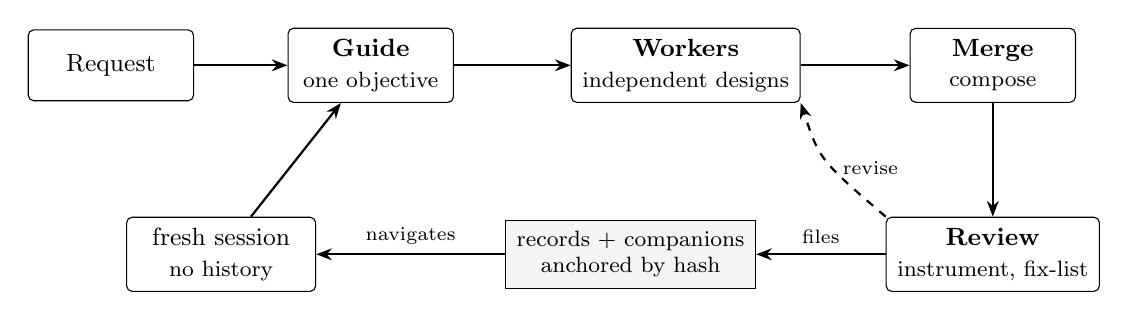
\begin{tikzpicture}[
  font=\small,
  b/.style={draw, rounded corners=2pt, align=center, inner sep=4pt, minimum height=9mm, minimum width=21mm},
  rec/.style={draw, fill=black!4, align=center, inner sep=4pt, font=\footnotesize, minimum width=30mm},
  arr/.style={-{Stealth[length=2mm]}, thick}
]
\node[b] (req) at (0,0) {Request};
\node[b] (guide) at (3.3,0) {\textbf{Guide}\\ \footnotesize one objective};
\node[b, minimum width=27mm] (panel) at (7.3,0) {\textbf{Workers}\\ \footnotesize independent designs};
\node[b] (merge) at (11.2,0) {\textbf{Merge}\\ \footnotesize compose};
\node[b, minimum width=27mm] (review) at (11.2,-2.4) {\textbf{Review}\\ \footnotesize instrument, fix-list};
\node[rec] (records) at (6.6,-2.4) {records + companions\\ \footnotesize anchored by hash};
\node[b, minimum width=24mm] (next) at (1.4,-2.4) {fresh session\\ \footnotesize no history};
\draw[arr] (req) -- (guide);
\draw[arr] (guide) -- (panel);
\draw[arr] (panel) -- (merge);
\draw[arr] (merge) -- (review);
\draw[arr] (review) -- node[above, font=\scriptsize] {files} (records);
\draw[arr] (records) -- node[above, font=\scriptsize] {navigates} (next);
\draw[arr] (next) -- (guide);
\draw[arr, dashed] (review.north west) .. controls (9.0,-1.2) .. node[right, font=\scriptsize, pos=0.4] {revise} (panel.south east);
\end{tikzpicture}
\caption{The loop. The review step is mandatory and runs on the design, before code; what it files is what a later historyless session navigates.}
\label{fig:loop}
\end{figure}

\section{Evaluation Protocol}
\label{sec:protocol}

A demonstration --- one arm, self-judged --- is not an experiment. Every pilot instantiates a frozen protocol or declares which part it waives.

\paragraph{Two questions, never merged.} \textbf{Q1:} when a product evolves through requirements nobody stated up front, does the method's arm end up architecturally better than an equally capable agent with no method, \emph{even when that agent may refactor freely at every step}? \textbf{Q2:} does a fresh session with no history continue correctly from the co-located records rather than re-deriving? Since a strong model refactors deeply, ``nicer code in one shot'' is explicitly not the bar.

\paragraph{Frozen package.} Identical starter for all arms; per-stage requirement cards revealed one at a time, where \emph{a card must not hint that a later stage exists} --- forward-looking language is a leak and disqualifies the run; a hidden staged spec plus canonical oracle answers the agents never see; visible per-stage acceptance and separate hidden probes derived only from already-revealed requirements; one equal cost ceiling per arm, against which a failed acceptance is charged rather than retried free.

\paragraph{Oracle policy.} The operator plays an ordinary product owner, not an architect: answers only from the current stage's hidden spec, volunteers nothing, never reveals a later requirement, defers technical choices an ordinary user would not make, and words answers neutrally --- one leak word (``still'', ``yet'', ``for now'') disqualifies the stage. Every question and verbatim answer is logged, and an identical question from another arm receives the identical answer.

\paragraph{Blind judging.} Artifacts are anonymized and relabelled, judges are isolated subagents that built nothing, mappings are sealed until after the reading. A verdict must turn on structural properties --- can an invariant be bypassed, is a boundary one seam or $N$ --- a removable local blemish must not flip it, and conversely a one-line funnel may be load-bearing rather than ceremony. Every load-bearing claim carries a reproduction or a precise \texttt{file:line}. Judges report per reading; readings are never merged into one score, a design win does not cancel a product loss, and $n=1$ per product is labelled suggestive, with strength claimed only from a sequence.

\section{Results}
\label{sec:results}

All results below were produced by the currently shipped method and principle documents. Studies 1--3 are design-and-change studies on fresh products or small modules, run once per arm per product; Study 4 runs three arms of three sessions each on a real, sizeable codebase. All arms and all judges are isolated subagents on the same model.

\subsection{Study 1: three products against a spec-driven baseline}

Two arms --- the shipped \aims{} skill run as-is including its mandatory review-and-revise round, and OpenSpec's own spec-first workflow --- on three products: a feed-ranking service, a booking-availability service, and an entitlements service. Design only, no code. Two dimensions scored separately: \textbf{D1}, first-round design quality on the stage-1 design; \textbf{D2}, change absorption after an unforeseen stage-2 requirement, read both through the instrument and through the rubric-free survival count (components reopened or discarded; lower is better).

\begin{table}[h]
\centering\small
\caption{Study 1. Three products, blind judges, sealed mappings. D2 carries two readings: the instrument's grade and the survival count, which needs no rubric to compute.}
\label{tab:study1}
\begin{tabular}{lcccccc}
\toprule
\multirow{2}{*}{Product} & \multicolumn{2}{c}{D1 (first round)} & \multicolumn{2}{c}{D2 (grade)} & D2 survival & Correctness \\
\cmidrule(lr){2-3}\cmidrule(lr){4-5}
 & \aims{} & OpenSpec & \aims{} & OpenSpec & (\aims{}/OS) & traps \\
\midrule
feed-ranking         & \best{10} & 8.5 & 9.9 & 8.5 & 0 / 0 \ (tie) & both passed all \\
booking-availability & \best{10} & 7.5 & \best{10} & 7.5 & $\approx$1 / $\approx$2 & both passed all \\
entitlements         & \best{10} & 8.5 & 9.9 & 8.5 & $\approx$2 / $\approx$2 \ (tie) & both passed all \\
\bottomrule
\end{tabular}
\end{table}

\paragraph{Where the gap is, and it is the same gap three times.} \aims{} wins first-round quality on all three products on one recurring axis: value objects and one-owner-per-rule. Its designs wrapped domain concepts in named types each with a single rule owner --- a bounded-interval type owning the half-open convention, a role type owning grant resolution, typed identifiers --- where the baseline's stage-1 designs carried bare floats, minute-scalars and positional strings. This is exactly the failure the principle document declares dominant (Section~\ref{sec:mechanism}, under-structuring), which is the point: the method's edge appears where its stated objective is, not diffusely.

\paragraph{The one trap that discriminated.} On booking, the new requirement made an existing rule gain a case. The baseline absorbed it by splitting the rule across a normal occupancy path and a separate trailing filter --- creating a second owner for one rule, a precondition failure under the instrument. \aims{} kept it to one owner, after its concept-fit pass caught the new concept being modelled as a synthetic instance of an existing entity. This is the mechanism of Consequence~2 firing on a real case: the cram was caught in the design, where it costs a paragraph.

\paragraph{Two readings here are not wins.} First, \textbf{both arms passed every hard correctness trap at both stages on all three products}. These products did not break a careful spec-first run; the traps discriminated on structure, not on raw correctness. A stronger falsifier is a product where the concept-cram is hard to avoid. Second, \textbf{\aims{} scored a perfect first-round grade on all three products}, and all three judges independently observed that its designs \emph{speak the rubric's own vocabulary}. Each judge controlled for this by crediting only structural, quoted findings, but the control is partial, and a perfect score everywhere is a problem independent of bias --- see Section~\ref{sec:threats}. The defensible claim is the narrower one: \emph{at least as good as the baseline on change absorption on all three, clearly better on first-round structure, and decisively better only where a structural trap discriminated.}

\paragraph{A product the method lost.} On a fourth product outside this set --- a feature-based identifier carried from plants to minerals across two staged reveals, judged blind by the same protocol --- the \aims{} arm \emph{lost} decisively to the baseline. Its type model (\texttt{Term $\mid$ Quantity}, a single point) could not represent an observed range the stage-2 card named (``6.5--7''), a precondition (S4) failure on exactly the full-input-space trap of Section~\ref{sec:principles}; the blind instrument scored the home arm below the baseline and marked it \textsc{blocked}. We record it for two reasons. It is the cleanest evidence the instrument is not a home referee: judged blind on its own form, it ranked the competitor above the method it was built for. And the defect is a \emph{design} fault the method's own concept-fit and full-input-space checks exist to catch --- caught here at review rather than prevented at design, the exact asymmetry Consequence~2 names. A wording change to the subtractive tie-break, prompted by the loss, was deliberately \emph{withheld} from the principle document and A/B-tested first on a further unseen product; it did not reproduce the over-cut and was not adopted, on the rule that a loss-prompted method change must prove itself on a product it has not seen before it is folded in.

\paragraph{Cost.} The \aims{} arms averaged roughly 140k tokens, 30--40 tool calls and 12 minutes per product; the baseline roughly 55k tokens, 4 tool calls and 3 minutes --- \textbf{2.5--3$\times$ the tokens and several times the wall-clock}. The spend goes on reading the principle set, filing records and running the mandatory revise round. Final design length was \emph{not} proportional to quality: the baseline's stage-2 documents were frequently the longer ones, so the extra cost buys structure rather than volume. Whether 3$\times$ is worth paying depends on how many future changes the design will absorb --- the quantity none of our studies is yet long enough to measure.

\subsection{Study 2: changing code that already exists}

Six experiments against a no-method control, using the brownfield principle set and its before-and-after measure, including one on a real open-source module rather than a synthetic one (Table~\ref{tab:study2}).

\begin{table}[h]
\centering\small
\caption{Study 2. ``Parity'' means both arms produced a correct, behaviour-preserving change.}
\label{tab:study2}
\begin{tabular}{llp{4.3cm}p{4.6cm}}
\toprule
\# & Codebase & Change & Reading \\
\midrule
1 & synthetic pricing & per-line tax + allocation, spelled out & parity; the card over-specified the trap \\
2 & synthetic $\times$3 & add operator / cancel event / discover allocation & parity; \aims{} cleaner (one owner vs.\ a scattered set) \\
3 & \textbf{real} open-source cache & add TTL across three entry paths + LRU override & parity (23 tests, 14-case oracle); \aims{} tighter --- expiry in the node, 31 vs.\ 53 lines \\
4 & synthetic pricing & three successive interacting changes & parity at each step; \best{\aims{} trajectory improves, control flat and denser} \\
5 & four-module ledger & multi-currency (cross-cutting) & parity, both on-grain; essentially a tie \\
6 & same code $\pm$ the record & fresh session adds a refund & both reused the owner, 14/14; record added legibility, \emph{not} a different outcome \\
\bottomrule
\end{tabular}
\end{table}

\paragraph{Correctness parity, everywhere.} On every task --- synthetic or real, single-file or cross-cutting --- a capable model with no method produced a correct, behaviour-preserving adaptation. The method never caught a bug the control shipped. We state the implication plainly because it bounds the claim: \emph{on a change a strong model can hold in one session, this method is not needed for correctness.}

\paragraph{The edge is a trajectory, and only a trajectory shows it.} Experiment~4 is load-bearing because of how it was measured: a before-and-after design review on the target's own grain, repeated across three successive interacting changes. The \aims{} arm improves at each step --- named single owners, short functions --- while the control stays flat and grows denser: an unnamed twenty-line block, a five-tuple read by a magic index. One change hides this completely; a sequence exposes it. This is the same phenomenon as the decay described in the introduction, observed under measurement: rot accumulates while every individual step works, which is precisely why a single-change benchmark cannot see it.

\paragraph{Consistency over dogma held.} Given a deliberately plain-style base, the method did \emph{not} impose value objects. It kept the bare-int grain and absorbed only the representation change the requirement forced. This is the answer to the obvious objection that a structure-favouring method will improve code into inconsistency, and it is a constraint the method states explicitly rather than an accident.

\paragraph{The continuity result is a partial null.} On a small, readable module a fresh session reconstructs the invariant from the code itself, so the co-located record added legibility and confidence but not a different outcome. The honest position on the record layer is therefore that it is load-bearing where the code is ambiguous or hides a rejected-alternative trap, at a scale where re-deriving is slow and error-prone --- a scale-and-longevity effect that none of our experiments is yet large enough to demonstrate in outcomes rather than in process.


\subsection{Study 3: a follow-up campaign}
\label{sec:study3}

A later campaign re-examined both claims with running code rather than design documents, under the same protocol: blind judges, sealed mappings, and each run's measure fixed before it ran --- with a prediction registered in advance where one is reported below. Its results sharpen the picture rather than change it.

\paragraph{Tests do not measure design.} Two designs passing the identical test suite scored 43 and 16 on the rubric, blind and from the code. Behavioural proxies fail in the same way: a capable model absorbed an unforeseen change with a three-line edit and no reopened owner while keeping a type-dispatch chain in place --- fewer edits, worse design. Only a change on the design's weak axis exposed the difference: type-dispatch builds reopened their engine when a new rule kind arrived (4 of 4), polymorphic builds added a class (0 of 2), at identical test results. We therefore treat a correctness gate as a floor that earns nothing and lead every design comparison with the rubric scored from the code; an earlier revision of our measurement policy, which led comparisons with behavioural proxies to escape the ceiling reported above, was itself a regression and was retracted.

\paragraph{The review, not the principles, carries the weight.} On four builds that pass every test but model a distinct concept as a data bag dispatched by type, the method's review flagged all four from the code alone, where the same principle stated in the implementing agent's prompt had not prevented them. On a weaker model the principle in the prompt changed nothing (2 of 6 builds took the shortcut either way); on a strong one, a single sentence of it made an unaided arm match the method. How often an unaided build takes a structural shortcut is model-dependent --- about one in six on one axis; none of three on a strong model and two of six on a weak one on another --- so the measurable benefit is a raised floor on that minority, and it did not compound across successive changes. No correctness gap appeared: unaided builds made no errors on two error-prone corners (0 of 12) nor on a deliberately designed interaction corner (0 of 6).

\paragraph{What the record holds that the code cannot.} Records filed by the method itself for a small module carried a non-goal (no targeting on a time window). A change request then contradicted it. All three agents given the records detected the contradiction and reconciled the record; none of three given only the code did, or could, since the non-goal appears nowhere in the code. The three is partly instruction-following; the zero is not. In the same run all six agents produced the same class hierarchy, with or without records: at this scale the design is recoverable from the code, and what is not recoverable is precisely what is absent from it. Relatedly, 62\% of a companion record the method filed before a placement rule existed restated the module's own docstrings --- duplicate state, the one part of a record that can go stale unaided. With the rule --- record only what the code cannot say --- an agent kept every item the code could not hold (6 of 6) and dropped every item it already carried (8 of 8), matching a prediction registered in advance.

\paragraph{A retraction worth reporting.} Six earlier record-layer runs in this campaign were withdrawn: the records in them had been written by the evaluator, to a model of the record layer the method does not have, so they tested that construction rather than the method. It is an instance of this paper's own thesis --- an instrument built by the party being evaluated measures that party --- and we report it for that reason.

\paragraph{Cost, second measurement.} 1.9--2.3$\times$ the tokens of an unaided build across two runs, and 3.7--12$\times$ the wall-clock, worst on small tasks, where the method's fixed overhead dominates.

\subsection{Study 4: design at scale}
\label{sec:study4}

Every earlier task was small enough for a strong model to find a good design unaided, so the method's central claim had not been tested where it matters. Study 4 used mkdocs (7,111 lines in 37 files, pinned commit) and three staged changes, each breaking an assumption the code already makes: multi-language sites (one language, one tree), correct incremental rebuilds across languages (a page depends only on its own file), and a self-contained offline export per language (one HTML file per page). \emph{A difficulty gate ran first}: four unaided agents built stage 1, and the task was kept only because their designs varied --- one clean, at least two with a reproduced precondition failure. A convergent task cannot separate two methods.

\paragraph{Design.} Three arms, three sessions each, a fresh session at every stage: A, the method with the records its earlier stages filed; B, the method with every record stripped; C, unaided. A and B share each stage-1 run, so they differ only in whether records reach later sessions. Goal 1 (design) is B against C, which isolates the method from its records; goal 2 (knowledge the code does not hold) has its own instrument. Blind judges of opposite disposition --- one weighting ownership, one simplicity, one scoring from code properties only --- graded every design on the full form, labels sealed by a committed hash; every S3 and S4 finding was reproduced against the code before unsealing, and none failed to reproduce.

\begin{table}[h]
\centering\footnotesize\setlength{\tabcolsep}{4pt}
\caption{Study 4: design grades (worst / mean of three sessions), blind. B vs C under the registered rule: supported if B's worst exceeds C's and the mean gap exceeds C's range.}
\label{tab:scale}
\begin{tabular}{llccc l}
\toprule
stage & judge & A (records) & B (records withheld) & C (unaided) & B vs C \\
\midrule
1 & 3 judges & \multicolumn{2}{c}{5.71--6.43 / 6.65--7.26} & 4.36--5.78 / 5.11--5.84 & method ahead, all three \\
2 & disjoint & 5.42 / 6.83 & 4.95 / 6.36 & 3.55 / 3.86 & supported \\
3 & ownership & 8.18 / 8.57 & 6.65 / 8.22 & 5.67 / 6.39 & no clear advantage \\
3 & simplicity & 4.73 / 5.73 & 6.26 / 7.13 & 4.69 / 5.04 & supported \\
3 & disjoint & 7.41 / 8.68 & 6.26 / 8.28 & 4.48 / 5.42 & supported \\
\bottomrule
\end{tabular}
\end{table}

\paragraph{Design: the method's designs scored higher at every stage.} At stage 3, the registered primary endpoint, two of three judges support B over C and the third finds no clear advantage; by the rule fixed in advance the panel verdict is \emph{supported}. The separating choices were visible in the code, not only in the grades: the method's designs more often kept the new concern behind one owner and a public seam, the unaided ones more often reached into existing modules' private functions and wrote a second owner of a rule. Reproduced precondition failures ran against the unaided arm at each stage --- 3 of 3 unaided sessions at stages 1 and 2, 2 of 3 at stage 3 under two judges --- while the method's arms had 0--2 of 3, once on a failure no unaided design made. The record did not change the design: A against B is mixed across judges, and the best single design of the nine came from B.

\paragraph{The verdict rests on a correction, and we report it first.} The stage-3 card carries a line --- open the file in the reader's own language --- that is the goal-2 trap: it contradicts the stage-1 legal non-goal, and the product owner withdrew it for every session that asked. The panel's first run scored that line as a design requirement; under it the one judge that finished would have \emph{falsified} the prediction, because the unaided designs that built language detection were credited for it. Scoring design without that line, in either direction, is what the protocol's separation of the two goals requires; the correction was made after seeing that judge's table and before unsealing, the whole panel was re-run, and both runs are published. Two floor-probe corrections made during the run are disclosed with what each changed; the floor enters no verdict.

\paragraph{The record, at scale.} Only the method's records carried the non-goal \emph{with its reason} (``a legal requirement in one market''). Every session given them stopped at the contradicting line and cited the record (3 of 3 sessions); with the records withheld, 2 of 3 sessions raised it --- one citing the product's user guide, one only asking how to implement it --- and unaided, 1 of 3. The three sessions that raised nothing are exactly the three whose exports detect the reader's language. By the rule we registered (the others at most 1 of 3) this is \emph{no clear advantage}, short by the one session that asked how rather than whether. No session that had the record failed to read it. The dissociation between the two goals is sharp: the best design of the nine was one of the three that built what the product's legal rule forbids.

\section{Why We Cannot Offer a Deterministic Benchmark}
\label{sec:measurement}

The reader will reasonably ask for an objective metric instead of a judged rubric. We ran the comparison where it was available. The continuation experiment produced the only pair of runnable implementations of the same task differing in a single design decision --- one returns a named type from its statement operation, the other a bare positional tuple, which a blind judge penalized as a data clump. Table~\ref{tab:radon} gives every deterministic metric we could compute alongside that judgement.

\begin{table}[h]
\centering\small
\caption{Deterministic static metrics against a blind design grade, two implementations of one task.}
\label{tab:radon}
\begin{tabular}{lcc}
\toprule
 & named type & bare tuple \\
\midrule
Blind design grade (0--4) & \best{4.0} & 3.5 \\
\midrule
Maintainability Index & 80.01 (A) & \best{80.50} (A) \\
Cyclomatic complexity (avg / max) & 2.07 / 4 & 2.07 / 4 \\
Halstead (volume / effort / difficulty) & 36 / 48 / 1.33 & 36 / 48 / 1.33 \\
SLOC & 36 & \best{27} \\
\bottomrule
\end{tabular}
\end{table}

Halstead is identical. Cyclomatic complexity is identical. Maintainability Index and SLOC \emph{favour} the design the judge graded lower, because a named type costs lines and adds no branches.

The metrics are not wrong. They measure surface complexity and volume --- a different construct from concept fit and abstraction quality --- and on this instance the two constructs are anti-correlated. This is $n=2$ on small files and is an illustration rather than a proof, but it generalizes in the direction one would predict: nearly every property that makes a design absorb the next requirement (a boundary that exists before it is strictly needed, a named concept, an explicit owner for an invariant) registers in a volume metric as \emph{cost}.

Three consequences follow. There is no available deterministic benchmark for the construct in question, and building one is not merely unfinished work --- the obvious candidates measure something else. Any evaluation of design quality is therefore an instrument of \emph{judgement}, whose validity rests on procedure: a specification-pinned inventory fixed before scoring, evidence required per score, sealed blinding, judges of opposing disposition, a reproduction for every load-bearing claim. And because judgement instruments can be captured in ways metrics cannot, the procedure must be adversarial by construction --- which is what Sections~\ref{sec:protocol} and~\ref{sec:threats} are for.

\section{Threats to Validity}
\label{sec:threats}

\paragraph{The judge and the method share a rubric (primary threat).} The judges grade against the same principle document the method designs toward. A method that encodes a rubric will score well on that rubric. Mitigations in force, none sufficient alone: the applicability set and the cited evidence are pinned to the specification rather than to the design (Figure~\ref{fig:instrument}), so a judge cannot select the requirements that flatter an arm; a reproduction is required for every load-bearing claim, which is what surfaced defects \emph{against} the method in earlier rounds of this work; and the survival count is reported separately because it needs no rubric to compute --- and there the reading is tie / win / tie, materially weaker than the graded one.

\paragraph{Vocabulary capture, observed.} All three judges independently noted that the method's designs speak the rubric's own vocabulary --- naming the subtractive pass, the tie-break falsifier, the concept-fit check. A judge sharing that rubric can be pulled toward a design that recites it. Each judge controlled for it by crediting only structural, quoted findings; the control is real and partial.

\paragraph{Ceiling effect.} The method scored a perfect first-round grade on all three products. Whatever the cause, an instrument that returns its maximum for one arm on every product has lost resolution for that arm: it can no longer register the next regression --- the single most valuable thing an instrument of this kind does. We read a rubric on which the method under test cannot lose as a rubric that needs a harder product, not as a result.

\paragraph{Lineage bias in LLM judging.} Where a judge and a contestant are drawn from the same model family, a margin can track that lineage's stylistic traits rather than the artifact's quality; we have observed this directly in earlier work on this system and the procedural remedy is to keep judge lineage disjoint from contestant lineage. This is a general hazard for LLM-as-judge evaluation~\cite{zheng2023judging} of agent-produced artifacts, where both sides come from a small pool.

\paragraph{$n=1$ per product.} Run-to-run variance for agent systems is real and visible. We report no win tally; the claim rests on an effect recurring across a sequence of products, and where a reading reverses we report the reversal rather than an average.

\paragraph{Single-axis readings reward the wrong thing.} A survival or change-locality count cannot see a correctness regression, and a design that reopens nothing may be reopening nothing precisely because it declined to build something required. Every locality reading in this work is therefore paired with a correctness gate, and we regard that pairing as mandatory for any future architectural benchmark.

\paragraph{External validity.} Three design products, all business-logic-shaped, plus small synthetic modules and one real open-source module for the adaptation work; design-only for Study~1; a single agent platform. Every codebase in Study~2 is small enough for one session to hold entirely --- which is exactly the regime in which the record layer is predicted \emph{not} to matter, so those parity results are neither evidence against the claim nor evidence for it. Study~4 is the one exception to that regime: a 7,000-line codebase and three successive changes, but a single codebase, three sessions per arm, and one model --- suggestive, and its final-stage verdict rests on a disclosed correction to the judges' specification. Nothing here speaks to systems where retrieval rather than reasoning dominates, or to concurrent multi-agent development.

\section{Discussion}

\paragraph{The mechanism argument is the transferable part.} If Section~\ref{sec:mechanism} is right, the requirements it derives --- a checkable predicate rather than an adjective, a check that fires at the design step, rationale externalized and staleness-flagged --- apply to any agent method, and a method can be assessed against them without reference to ours. The empirical results are consistent with the argument in a specific and falsifiable way: the method's measured advantage appears on exactly the axis its document names dominant (under-structuring: value objects, one owner per rule), and its one decisive win came from a check firing in the design rather than in review.

\paragraph{What the results do not support.} They do not support a correctness advantage on changes a strong model handles in one session --- six experiments say the opposite, plainly. They support the record layer in one outcome only --- a declared non-goal, detected when a change contradicts it (Sections~\ref{sec:study3} and~\ref{sec:study4}) --- and at scale that outcome fell one session short of the threshold we registered; the record did not change a design, at any scale. And they do not support a claim of general superiority: a perfect score on three products against a shared rubric is a measurement ceiling, not a verdict.

\paragraph{Scale: a first test, and what remains.} The method's central bet --- that structure compounds and rationale accumulates --- predicts an effect that grows with the size of the codebase and the number of independent sessions touching it. Study~4 is the first test on a real codebase with changes that cut across it, and it points the predicted way on design, three stages running. What it cannot settle: three sessions per arm, one codebase, judges who share the rubric's lineage, and a final verdict carried by two judges of three. A longer sequence, on a codebase no session can hold, with a judge outside that lineage and more kinds of recorded intent than one non-goal, is the experiment that would.

\section{Conclusion}

A language model optimizes the goal it is given. Under a loop that terminates on correctness, structure is not a goal, and the model's prior --- ordinary working code --- is what fills the gap; the rationale for whatever structure does appear is discarded when the session ends. \aims{} addresses each of those three facts directly: it states structure as a checkable document, runs the check inside the design step before the artifact conditions the rest of generation, and files the conclusion beside the code for the next historyless session.

Measured against a spec-driven baseline on three fresh products, this wins first-round design quality on all three on a single recurring axis, ties or wins change absorption on a rubric-free count, costs 2--3$\times$, and passes no correctness trap the baseline failed. Measured on six adaptation tasks, it produces no correctness advantage at all; its edge is a design trajectory visible only across a sequence. On a real 7,000-line codebase with three cross-cutting changes, its designs scored above unaided ones at every stage under blind judges, with its records withheld; the records themselves carried the one thing the code could not --- a legal non-goal and its reason --- to every session that had them. Two of its strongest-looking numbers we report as instrument failures rather than results.

The finding we hold most firmly is the least flattering: there is no deterministic benchmark for what this work is trying to improve, the classical metrics that resemble one are anti-correlated with it on the only data where we could compare, and the judged instruments that replace them are only as sound as the adversarial procedure around them. The protocol, the principle documents, the sealed mappings and all run logs are published, and a well-run refutation would be a good outcome.

\section*{Availability}
Method, frozen experiment packages, run logs, judge reports and sealed blind mappings: \url{https://github.com/eliezeravihail/aims}.

\begin{thebibliography}{99}
\small
\bibitem{amodei2016concrete} D.~Amodei, C.~Olah, J.~Steinhardt, P.~Christiano, J.~Schulman and D.~Mané. Concrete problems in AI safety. \emph{arXiv:1606.06565}, 2016.
\bibitem{austin2021program} J.~Austin et al. Program synthesis with large language models. \emph{arXiv:2108.07732}, 2021.
\bibitem{beck2012tweet} K.~Beck. ``For each desired change, make the change easy (warning: this may be hard), then make the easy change.'' Twitter/X, 2012.
\bibitem{brown2020language} T.~B. Brown et al. Language models are few-shot learners. \emph{NeurIPS}, 2020.
\bibitem{chen2021codex} M.~Chen et al. Evaluating large language models trained on code. \emph{arXiv:2107.03374}, 2021.
\bibitem{chidamber1994metrics} S.~R. Chidamber and C.~F. Kemerer. A metrics suite for object oriented design. \emph{IEEE Trans.\ Software Engineering}, 20(6):476--493, 1994.
\bibitem{coleman1994using} D.~Coleman, D.~Ash, B.~Lowther and P.~Oman. Using metrics to evaluate software system maintainability. \emph{Computer}, 27(8):44--49, 1994.
\bibitem{feathers2004working} M.~Feathers. \emph{Working Effectively with Legacy Code}. Prentice Hall, 2004.
\bibitem{fowler2018refactoring} M.~Fowler. \emph{Refactoring: Improving the Design of Existing Code}. 2nd ed., Addison-Wesley, 2018.
\bibitem{halstead1977elements} M.~H. Halstead. \emph{Elements of Software Science}. Elsevier, 1977.
\bibitem{hong2024metagpt} S.~Hong et al. MetaGPT: Meta programming for a multi-agent collaborative framework. \emph{ICLR}, 2024.
\bibitem{jimenez2024swebench} C.~E. Jimenez et al. SWE-bench: Can language models resolve real-world GitHub issues? \emph{ICLR}, 2024.
\bibitem{knuth1984literate} D.~E. Knuth. Literate programming. \emph{The Computer Journal}, 27(2):97--111, 1984.
\bibitem{krakovna2020specification} V.~Krakovna et al. Specification gaming: the flip side of AI ingenuity. DeepMind blog, 21 April 2020.
\bibitem{liu2024lost} N.~F. Liu et al. Lost in the middle: How language models use long contexts. \emph{TACL}, 12:157--173, 2024.
\bibitem{madaan2023selfrefine} A.~Madaan et al. Self-Refine: Iterative refinement with self-feedback. \emph{NeurIPS}, 2023.
\bibitem{manheim2019categorizing} D.~Manheim and S.~Garrabrant. Categorizing variants of Goodhart's law. \emph{arXiv:1803.04585}, 2018.
\bibitem{martin2003agile} R.~C. Martin. \emph{Agile Software Development: Principles, Patterns, and Practices}. Prentice Hall, 2003.
\bibitem{mccabe1976complexity} T.~J. McCabe. A complexity measure. \emph{IEEE Trans.\ Software Engineering}, SE-2(4):308--320, 1976.
\bibitem{nygard2011adr} M.~Nygard. Documenting architecture decisions. Technical note, 2011.
\bibitem{ouyang2022training} L.~Ouyang et al. Training language models to follow instructions with human feedback. \emph{NeurIPS}, 2022.
\bibitem{parnas1972criteria} D.~L. Parnas. On the criteria to be used in decomposing systems into modules. \emph{Comm.\ ACM}, 15(12):1053--1058, 1972.
\bibitem{qian2024chatdev} C.~Qian et al. ChatDev: Communicative agents for software development. \emph{ACL}, 2024.
\bibitem{sharma2023sycophancy} M.~Sharma et al. Towards understanding sycophancy in language models. \emph{arXiv:2310.13548}; \emph{ICLR}, 2024.
\bibitem{shinn2023reflexion} N.~Shinn et al. Reflexion: Language agents with verbal reinforcement learning. \emph{NeurIPS}, 2023.
\bibitem{vaswani2017attention} A.~Vaswani et al. Attention is all you need. \emph{NeurIPS}, 2017.
\bibitem{wu2023autogen} Q.~Wu et al. AutoGen: Enabling next-gen LLM applications via multi-agent conversation. \emph{arXiv:2308.08155}, 2023.
\bibitem{yang2024sweagent} J.~Yang et al. SWE-agent: Agent-computer interfaces enable automated software engineering. \emph{NeurIPS}, 2024.
\bibitem{yao2023react} S.~Yao et al. ReAct: Synergizing reasoning and acting in language models. \emph{ICLR}, 2023.
\bibitem{zheng2023judging} L.~Zheng et al. Judging LLM-as-a-judge with MT-Bench and Chatbot Arena. \emph{NeurIPS}, 2023.
\end{thebibliography}

\end{document}
